% UTF-8 encoding
% Compile with latex+dvipdfmx, pdflatex, xelatex or lualatex

\documentclass[hyperref, UTF8]{ctexart}
\usepackage{amssymb}
\usepackage{amsmath}
\usepackage{graphicx}
\usepackage{subfigure}
\usepackage{geometry}
\usepackage{caption}
\usepackage{upgreek}
\newcommand{\under}[1]{\frac{1}{#1}}
\newcommand{\underpone}[1]{\frac{#1}{1+#1}}
\newcommand{\volt}{{\rm V}}
\newcommand{\source}{{\rm S}}
\newcommand{\second}{{\rm s}}
\newcommand{\radian}{{\rm rad}}
\newcommand{\ampere}{{\rm A}}
\newcommand{\milliampere}{{\rm mA}}
\newcommand{\microampere}{{\rm \upmu A}}
\newcommand{\hertz}{{\rm Hz}}
\newcommand{\kilohertz}{{\rm kHz}}
\newcommand{\megahertz}{{\rm MHz}}
\newcommand{\gigahertz}{{\rm GHz}}
\newcommand{\ohm}{\Omega}
\newcommand{\kiloohm}{{\rm k}\Omega}
\newcommand{\watt}{{\rm W}}
\newcommand{\kilowatt}{{\rm kW}}
\newcommand{\degree}{^{\circ}}
\newcommand{\farad}{{\rm F}}
\newcommand{\microfarad}{{\rm \upmu F}}
\newcommand{\millifarad}{{\rm mF}}
\newcommand{\henry}{{\rm H}}
\newcommand{\J}{{\rm j}}
\newcommand{\D}{{\rm d}}
\newcommand{\E}{{\rm e}}

\title{电子学基础——第十一次作业}
\author{LXQ}
\date{2019.12.20}

\geometry{left=2.0cm, right=2.0cm, top=2.5cm, bottom=2.5cm}
\linespread{1}

\begin{document}

\maketitle

\paragraph{11.4} \label{11.4}
    Construct the Bode plot of $|V_{out}/V_{in}|$ for the stages depicted in Fig. 11-62.

    \begin{figure}[!htb]
        \centering
        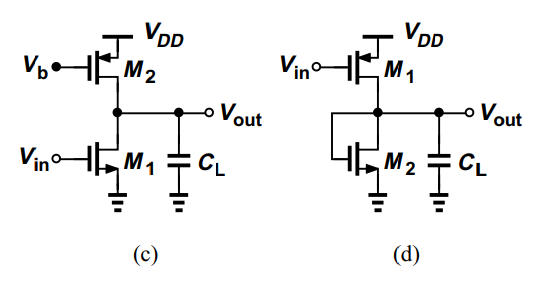
\includegraphics[width=0.362\textwidth]{p11-62.png}
        \caption*{Figure 11-62}
    \end{figure}

\paragraph{解}
    (c) $M_2$电流稳定,可视为$r_{o1}$电阻。则
    $$A_0 = -g_m(r_{o2}//r_{o1}), \omega_p = \under{r_{o2}C_L}$$
    波特图如图 p11-4-c 所示。

    (d) $M_2$可视为$\under{g_{m2}}$,则有极点$\omega_p = \frac{g_{m2}}{C_L}$
    $$A_0 = -\frac{g_{m1}}{g_{m2}}$$
    波特图如图 p11-4-d。

    \begin{figure}[!htb]
        \centering
        \begin{minipage}[t]{0.259\textwidth}
        \centering
        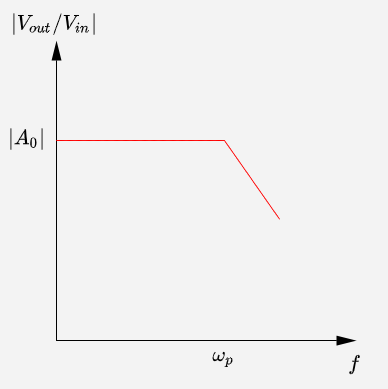
\includegraphics[width=1\textwidth]{p11-4-c-sol.png}
        \caption*{(a)}
        \end{minipage}
        \begin{minipage}[t]{0.259\textwidth}
        \centering
        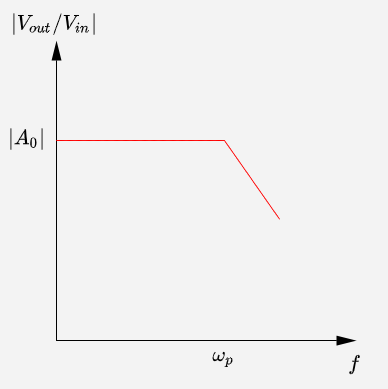
\includegraphics[width=1\textwidth]{p11-4-d-sol.png}
        \caption*{(b)}
        \end{minipage}
        \caption*{Figure p11-4}
    \end{figure}    

\paragraph{11.6} \label{11.6}
    An amplifier exihibits two poles at $100\megahertz$ and $10\gigahertz$ and a zero at $1\gigahertz$. Construct the Bode plot of $|V_{out}/V_{in}|$.

\paragraph{解}
    如图 p11-6 所示。其中三个斜率发生改变的点为$\omega_{p1} = 100 \megahertz$, $\omega_{z} = 1\gigahertz$, $\omega_{p2} = 10\gigahertz$.

    \begin{figure}[!htb]
        \centering
        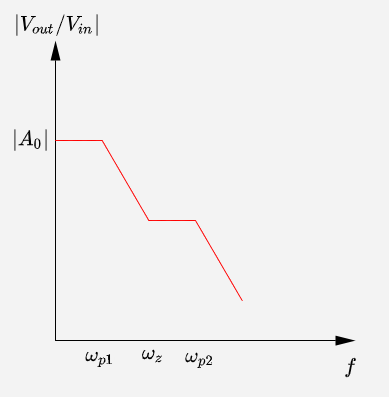
\includegraphics[width=0.259\textwidth]{p11-6-sol.png}
        \caption*{Figure p11-6}
    \end{figure}

\paragraph{11.12} \label{11.12}
    Due to a mannufacturing error, a parasitic resistance $R_P$ has appeared in series with the source of $M_1$ in Fig. 11-65. Assuming $\lambda = 0$ and neglecting other capacitances, determine the input and output poles of the circuit.

    \begin{figure}[!htb]
        \centering
        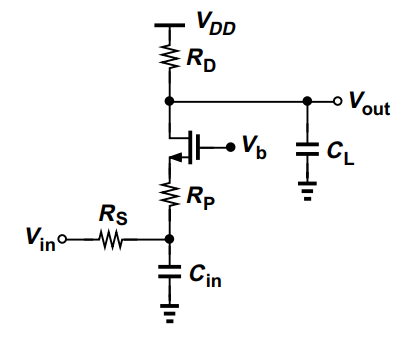
\includegraphics[width=0.268\textwidth]{p11-65.png}
        \caption*{Figure 11-65}
    \end{figure}

\paragraph{解}

    \begin{figure}[!htb]
        \centering
        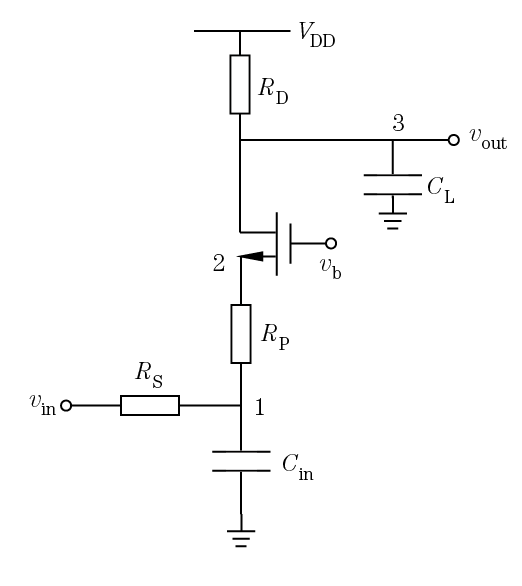
\includegraphics[width=0.348\textwidth]{p11-12-sol.png}
        \caption*{Figure p11-12}
    \end{figure}
    
    如图 p11-12 所示。对于节点一,
    $$\omega_{p1} = \under{C_{in}[R_S // (R_P + \under{g_m})]}$$
    
    节点二仅有分压效果,不产生极点。

    对于节点三,
    $$\omega_{p2} = \under{C_LR_D}$$

\paragraph{11.13} \label{11.13}
    Repeat Problem 12 for the circuit shown in Fig. 11-66.

    \begin{figure}[!htb]
        \centering
        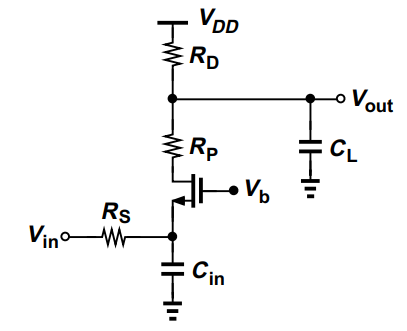
\includegraphics[width=0.271\textwidth]{p11-66.png}
        \caption*{Figure 11-66}
    \end{figure}

\paragraph{解}
    在输入端,
    $$\omega_{p1} = \under{C_{in}(R_S // \under{g_m})}$$
    在输出端,
    $$\omega_{p2} = \under{C_L(R_D // R_P)}$$

\paragraph{11.14} \label{11.14}
    Repeat Problem 12 for the CS stage depicted in Fig. 11-67.

    \begin{figure}[!htb]
        \centering
        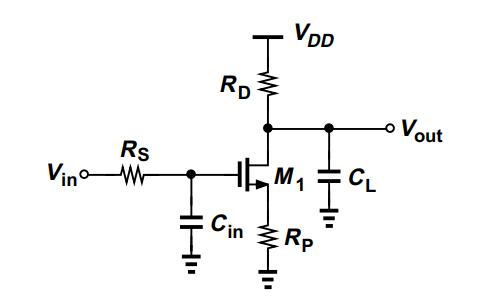
\includegraphics[width=0.319\textwidth]{p11-67.png}
        \caption*{Figure 11-67}
    \end{figure}

\paragraph{解}
    在输入端,
    $$\omega_{p1} = \under{C_{in}R_S}$$
    在输出端,
    $$\omega_{p2} = \under{C_LR_D}$$

\paragraph{11.19} \label{11.19}
    Using Miller's theorem, estimate the input capacitance of the circuit depicted in Fig. 11-71. Assume $\lambda > 0$ but neglect other capacitances. What happens if $\lambda \to 0$?

    \begin{figure}[!htb]
        \centering
        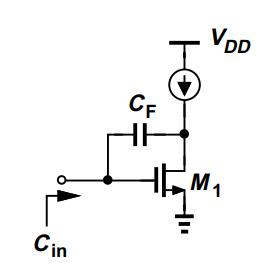
\includegraphics[width=0.187\textwidth]{p11-71.png}
        \caption*{Figure 11-71}
    \end{figure}

\paragraph{解}
    $M_1$内部可看作并联电阻$r_o$,则在小信号电路中可看作$r_o$连接漏端与地,从而可对$C_F$应用密勒定理。
    $$C_{in} = (1+g_mr_o)C_F$$
    当$\lambda \to 0$,则$C_{in} \to \infty$

\paragraph{11.38} \label{11.38}
    Assuming $\lambda > 0$ and using Miller's theorem, determine the input and output poles of the stages depicted in Fig. 11-80.

    \begin{figure}[!htb]
        \centering
        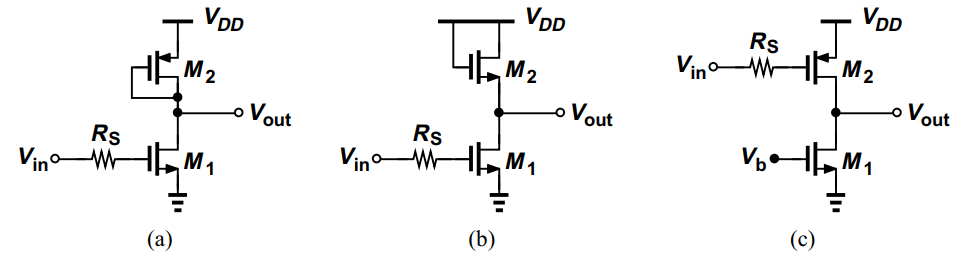
\includegraphics[width=0.646\textwidth]{p11-80.png}
        \caption*{Figure 11-80}
    \end{figure}

\paragraph{解}
    (a) 画出所有电容的电路以及简化后的电路如图 p11-38-a 所示。其中
    \begin{figure}[!htb]
        \centering
        \begin{minipage}[t]{0.397\textwidth}
        \centering
        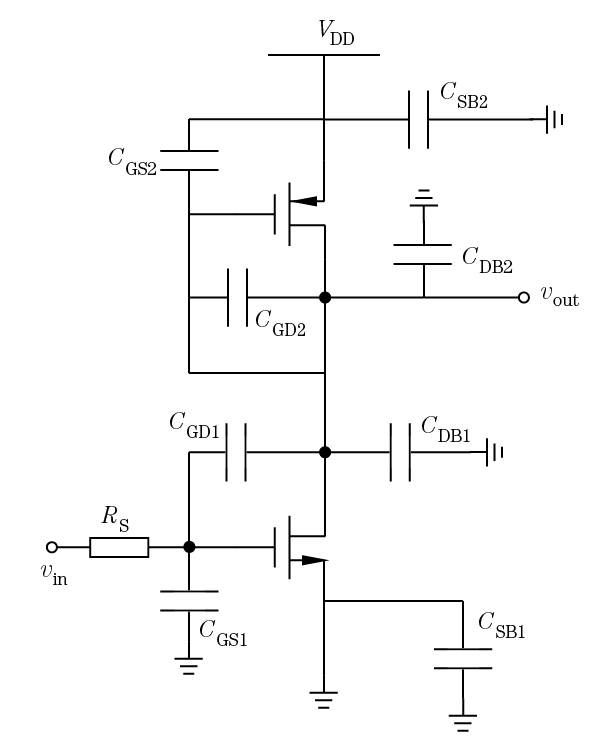
\includegraphics[width=1\textwidth]{p11-38-a-sol1.png}
        \caption*{(1) 标出电容}
        \end{minipage}
        \begin{minipage}[t]{0.442\textwidth}
        \centering
        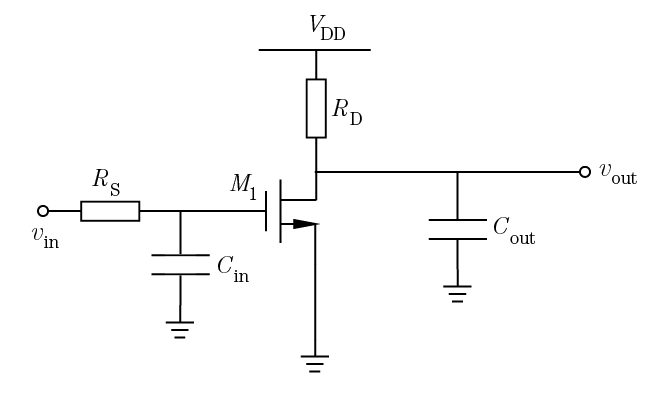
\includegraphics[width=1\textwidth]{p11-38-a-sol2.png}
        \caption*{(2) 简化电路}
        \end{minipage}
        \caption*{Figure p11-38-a}
    \end{figure}        
    \begin{align*}
        R_D & = \under{g_{m2}}//r_{o2} \\
        A_0 & = g_{m1}\left(\under{g_{m2}}//r_{o2}//r_{o1}\right) \\
        C_{in} & = C_{GS1} + C_{GD1}\left(1+g_{m1}\left(\under{g_{m2}}//r_{o2}//r_{o1}\right)\right) \\
        C_{out} & = C_{DB1}+C_{DB2}+C_{GS2}+C_{GD1}\left[1+\under{g_{m1}\left(\under{g_{m1}} // r_{o2} // r_{o1}\right)}\right]
    \end{align*}
    其中$A_0$为电路低频增益,从而
    \begin{align*}
        \omega_{p1} & = \left[R_S \left[ C_{GS1} + C_{GD1}\left(1+g_{m1}\left(\under{g_{m2}}//r_{o2}//r_{o1}\right)\right)\right] \right] ^ {-1} \\
        \omega_{p2} & = \left[\left(\under{g_{m2}} // r_{o2}\right)\left[C_{DB1}+C_{DB2}+C_{GS2}+C_{GD1}\left(1+\under{g_{m1}\left(\under{g_{m1}} // r_{o2} // r_{o1}\right)}\right)\right]\right] ^ {-1}
    \end{align*}

    (b) 画出所有电容后的电路以及简化后的电路如图 p11-38-b 所示。其中
    \begin{figure}[!htb]
        \centering
        \begin{minipage}[t]{0.413\textwidth}
        \centering
        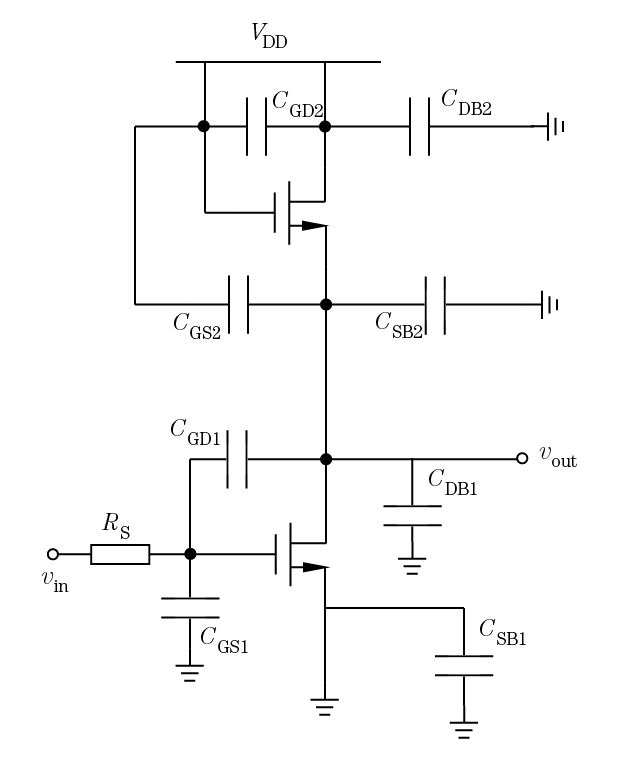
\includegraphics[width=1\textwidth]{p11-38-b-sol1.png}
        \caption*{(1) 标出电容}
        \end{minipage}
        \begin{minipage}[t]{0.401\textwidth}
        \centering
        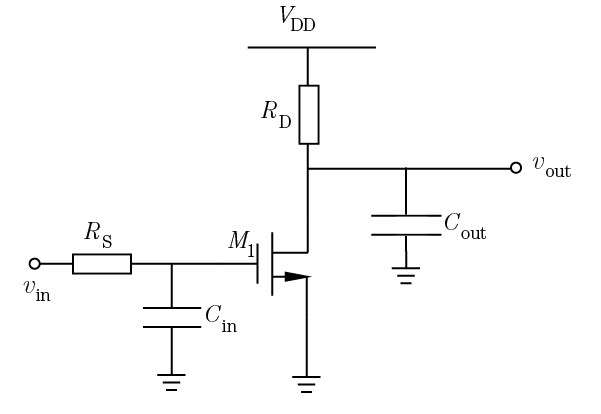
\includegraphics[width=1\textwidth]{p11-38-b-sol2.png}
        \caption*{(2) 简化电路}
        \end{minipage}
        \caption*{Figure p11-38-b}
    \end{figure}        
    \begin{align*}
        R_D & = \under{g_{m2}} // r_{o2} \\
        A_0 & = g_{m1}\left(\under{g_{m2}} // r_{o2} // r_{o1} \right) \\
        C_{in} & = C_{GS1}+C_{GD1}\left[1 - g_{m1}\left(\under{g_{m2}} // r_{o2} // r_{o1} \right)\right] \\
        C_{out} & = C_{DB1} + C_{GS2} + C_{SB2} + C_{GD1}\left[1 - \under{g_{m1}\left(\under{g_{m2}} // r_{o2} // r_{o1} \right)}\right]
    \end{align*}
    其中$A_0$为电路低频增益,从而
    \begin{align*}
        \omega_{p1} & = \left[ R_S
        \left[C_{GS1}+C_{GD1}\left(1 - g_{m1}\left(\under{g_{m2}} // r_{o2} // r_{o1} \right)\right) \right] \right] ^ {-1} \\
        \omega_{p2} & = \left[ 
            \left( \under{g_{m2}}//r_{o2}\right) 
            \left[ C_{DB1} + C_{GS2} + C_{SB2} + C_{GD1}\left(1 - \under{g_{m1}\left(\under{g_{m2}} // r_{o2} // r_{o1} \right)}\right) \right] 
            \right] ^ {-1}
    \end{align*}

    (c) 画出所有电容后的电路以及简化后的电路如图 p11-38-c 所示。其中
    \begin{figure}[!htb]
        \centering
        \begin{minipage}[t]{0.385\textwidth}
        \centering
        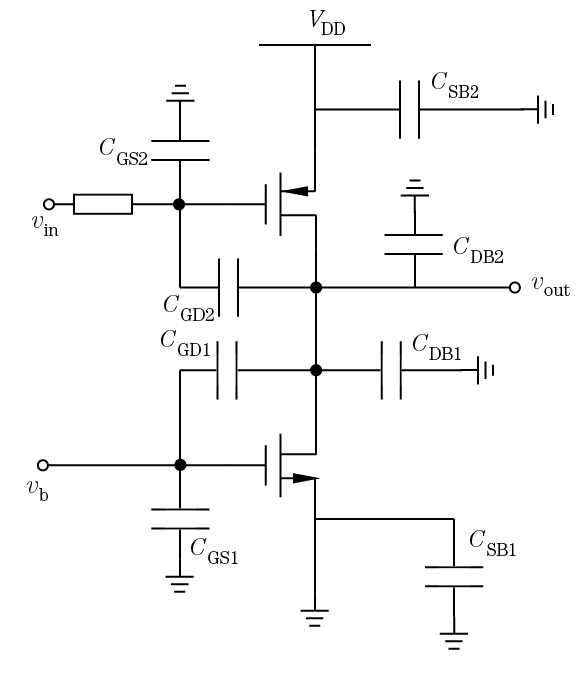
\includegraphics[width=1\textwidth]{p11-38-c-sol1.png}
        \caption*{(1) 标出电容}
        \end{minipage}
        \begin{minipage}[t]{0.383\textwidth}
        \centering
        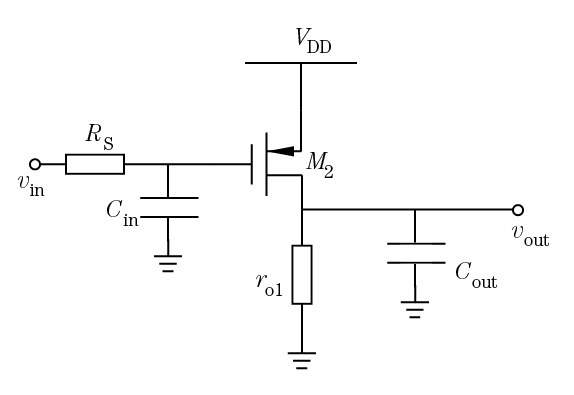
\includegraphics[width=1\textwidth]{p11-38-c-sol2.png}
        \caption*{(2) 简化电路}
        \end{minipage}
        \caption*{Figure p11-38-c}
    \end{figure}
    \begin{align*}
        A_0 & = - g_{m1}\left(r_{o2} // r_{o1} \right) \\
        C_{in} & = C_{GS2}+C_{GD2}\left[1 + g_{m1}\left(r_{o2} // r_{o1} \right)\right] \\
        C_{out} & = C_{DB1} + C_{DB2} + C_{GD1} + C_{GD2}\left[1 + \under{g_{m1}\left(r_{o2} // r_{o1} \right)}\right]
    \end{align*}
    其中$A_0$为电路低频增益,从而
    \begin{align*}
        \omega_{p1} & = \left[ R_S
        \left[ C_{GS2}+C_{GD2}\left(1 + g_{m1}\left(r_{o2} // r_{o1} \right)\right) \right] 
        \right] ^ {-1} \\
        \omega_{p2} & = \left[ 
            r_{o1}
            \left[ C_{DB1} + C_{DB2} + C_{GD1} + C_{GD2}\left(1 + \under{g_{m1}\left(r_{o2} // r_{o1} \right)}\right) \right] 
            \right] ^ {-1}
    \end{align*}

\paragraph{11.42} \label{11.42}
    The circuit depicted in Fig. 11-82 is called ana "active inductor". Neglcting other capacitances and assuming $\lambda = 0$, compute $Z_{in}$. Use Bode's rule to plot $|Z_{in}|$ as a function of frequency and explain why it exhibits inductive behavior.

    \begin{figure}[!htb]
        \centering
        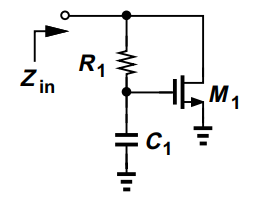
\includegraphics[width=0.170\textwidth]{p11-82.png}
        \caption*{Figure 11-82}
    \end{figure}

\paragraph{解}
    $$Z_{in} = (R_1 - \J \under{\omega C_1}) // \under{g_{m}} = \under{g_{m}} \cdot \frac{1+\J \omega R_1 C_1}{1 + \J \omega C_1(\under{g_m}+R_1)}$$
    $$\omega_z = \under{R_1C_1}, \omega_p = \under{C_1(\under{g_m}+R_1)}$$
    从而可作波特图如图 p11-42 所示,在高频下$|Z_{in}|$更小,显出电导性。

    \begin{figure}[!htb]
        \centering
        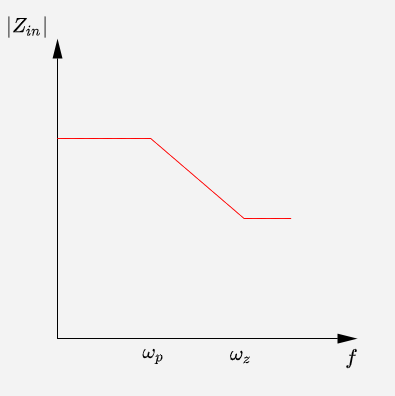
\includegraphics[width=0.263\textwidth]{p11-42-sol.png}
        \caption*{Figure p11-42}
    \end{figure}
    
\paragraph{11.46} \label{11.46}
    Determine the transfer function of the circuits shown in Fig. 11-86. Assume $\lambda = 0$ for $M_1$.

    \begin{figure}[!htb]
        \centering
        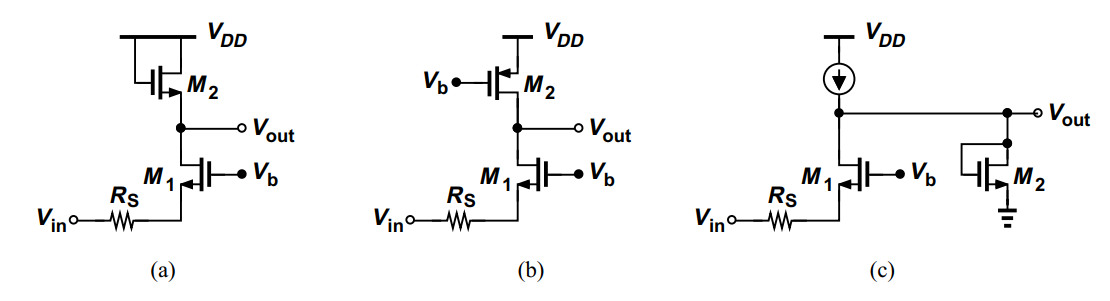
\includegraphics[width=0.740\textwidth]{p11-86.png}
        \caption*{Figure 11-86}
    \end{figure}

\paragraph{解}
    (a) 画出所有电容后的电路以及简化后的电路如图 p11-46-a 所示。其中
    \begin{figure}[!htb]
        \centering
        \begin{minipage}[t]{0.481\textwidth}
        \centering
        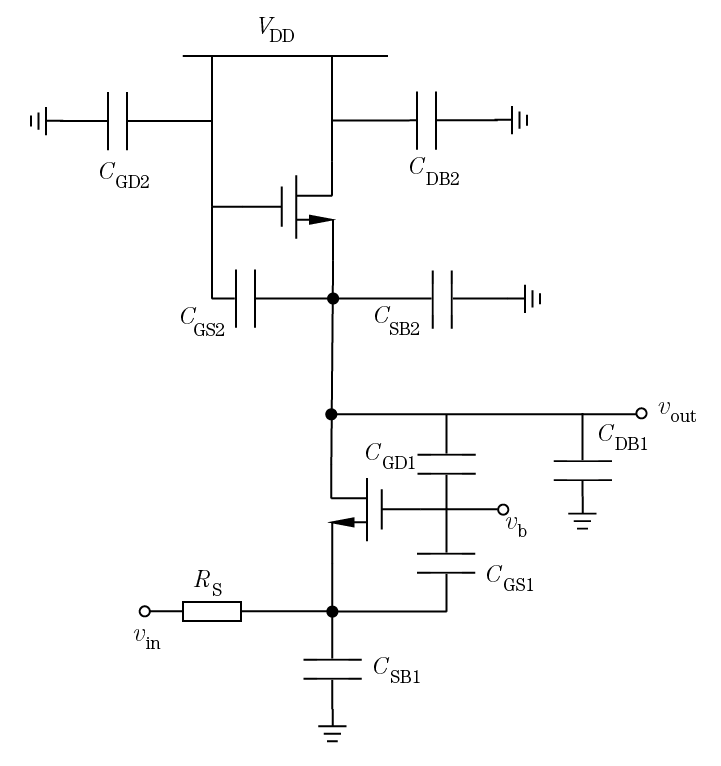
\includegraphics[width=1\textwidth]{p11-46-a-sol1.png}
        \caption*{(1) 标出电容}
        \end{minipage}
        \begin{minipage}[t]{0.408\textwidth}
        \centering
        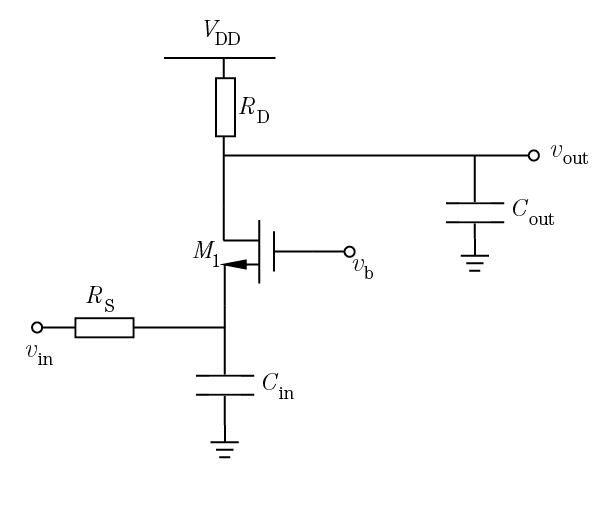
\includegraphics[width=1\textwidth]{p11-46-a-sol2.png}
        \caption*{(2) 简化电路}
        \end{minipage}
        \caption*{Figure p11-46-a}
    \end{figure}        
    \begin{align*}
        R_D & = \under{g_{m2}} // r_{o2} \\
        A_0 & = g_{m1}(\under{g_{m2}}//r_{o2}) \\
        C_{in} & = C_{SB1}+C_{GS1} \\
        C_{out} & = C_{DB1}+C_{DB2}+C_{GD2}+C_{GD1}
    \end{align*}
    其中$A_0$为电路低频增益,从而
    \begin{align*}
        \omega_{p1} & = \left[ R_S 
            (C_{SB1}+C_{GS1})
            \right] ^ {-1} \\
        \omega_{p2} & = \left[ \left(\under{g_{m2}} // r_{o2} \right)
            (C_{DB1}+C_{DB2}+C_{GD2}+C_{GD1})
            \right] ^ {-1}\\
        A & = \frac{A_0}{
            \left( 1 + \frac{\J \omega}{\omega_{p1}}
            \right)
            \left( 1 + \frac{\J \omega}{\omega_{p2}} \right)
        } \\
        & = \frac{g_{m1}(\under{g_{m2}}//r_{o2})}{
            \left[ 1 + \J \omega R_S 
            (C_{SB1}+C_{GS1}) \right]
            \left[ 1 + \J \omega \left(\under{g_{m2}} // r_{o2}\right)
            (C_{DB1}+C_{DB2}+C_{GD2}+C_{GD1}) \right]
        }
    \end{align*}

    (b) 画出所有电容后的电路以及简化后的电路如图 p11-46-b 所示。其中
    \begin{figure}[!htb]
        \centering
        \begin{minipage}[t]{0.439\textwidth}
        \centering
        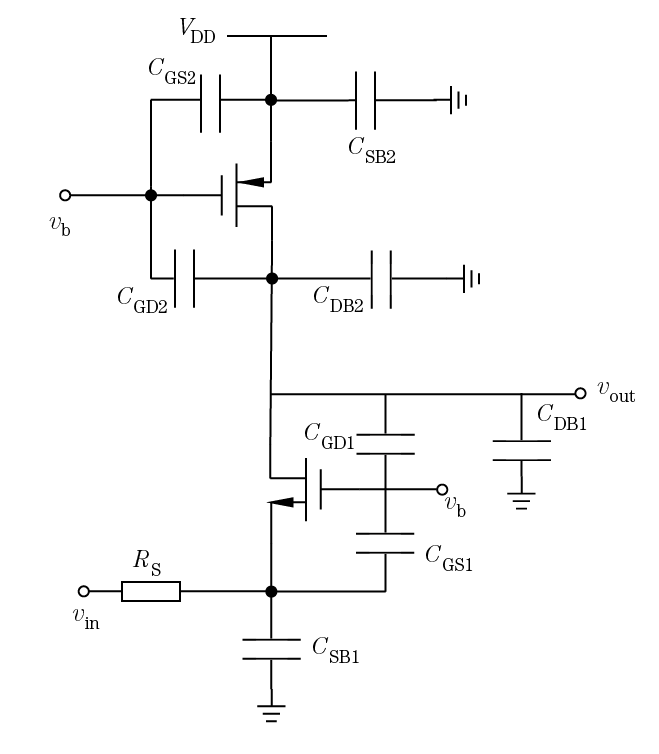
\includegraphics[width=1\textwidth]{p11-46-b-sol1.png}
        \caption*{(1) 标出电容}
        \end{minipage}
        \begin{minipage}[t]{0.400\textwidth}
        \centering
        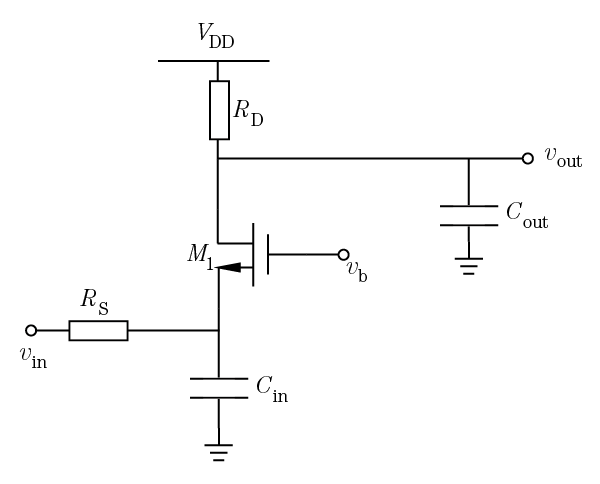
\includegraphics[width=1\textwidth]{p11-46-b-sol2.png}
        \caption*{(2) 简化电路}
        \end{minipage}
        \caption*{Figure p11-46-b}
    \end{figure}
    \begin{align*}
        A_0 & = g_{m1}r_{o2} \\
        C_{in} & = C_{SB1}+C_{GS1} \\
        C_{out} & = C_{DB1}+C_{DB2}+C_{GD2}+C_{GD1}
    \end{align*}
    其中$A_0$为电路低频增益,从而
    \begin{align*}
        \omega_{p1} & = \left[ R_S 
            (C_{SB1}+C_{GS1})
            \right] ^ {-1} \\
        \omega_{p2} & = \left[ r_{o2}
            (C_{DB1}+C_{DB2}+C_{GD2}+C_{GD1})
            \right] ^ {-1}\\
        A & = \frac{A_0}{
            \left( 1 + \frac{\J \omega}{\omega_{p1}}
            \right)
            \left( 1 + \frac{\J \omega}{\omega_{p2}} \right)
        } \\
        & = \frac{g_{m1}r_{o2}}{
            \left[ 1 + \J \omega R_S 
            (C_{SB1}+C_{GS1}) \right]
            \left[ 1 + \J \omega r_{o2}
            (C_{DB1}+C_{DB2}+C_{GD2}+C_{GD1}) \right]
        }
    \end{align*}

    (c) 画出所有电容后的电路以及简化后的电路如图 p11-46-c 所示。其中
    \begin{figure}[!htb]
        \centering
        \begin{minipage}[t]{0.577\textwidth}
        \centering
        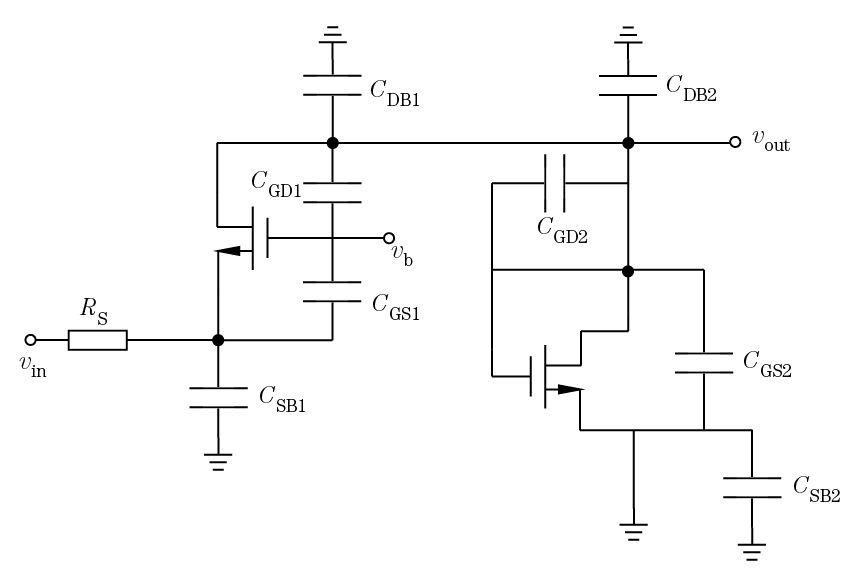
\includegraphics[width=1\textwidth]{p11-46-c-sol1.png}
        \caption*{(1) 标出电容}
        \end{minipage} \\
        \begin{minipage}[t]{0.424\textwidth}
        \centering
        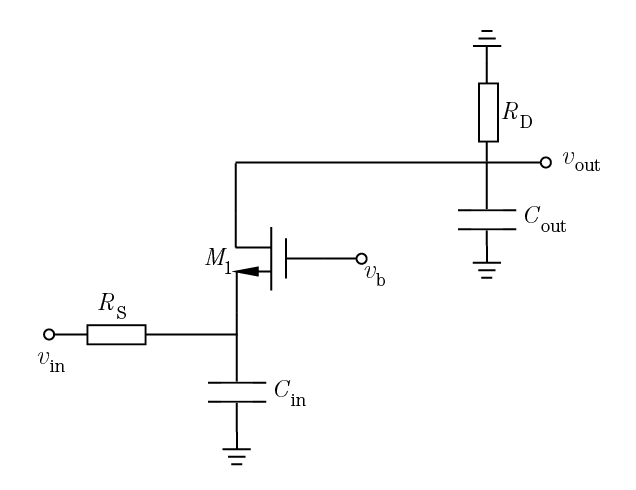
\includegraphics[width=1\textwidth]{p11-46-c-sol2.png}
        \caption*{(2) 简化电路}
        \end{minipage}
        \caption*{Figure p11-46-c}
    \end{figure}        
    \begin{align*}
        R_D & = \under{g_{m2}} // r_{o2} \\
        A_0 & = g_{m1}\left(\under{g_{m2}} // r_{o2}\right) \\
        C_{in} & = C_{SB1}+C_{GS1} \\
        C_{out} & = C_{DB1}+C_{DB2}+C_{GS2}+C_{GD1}
    \end{align*}
    其中$A_0$为电路低频增益,从而
    \begin{align*}
        \omega_{p1} & = \left[ R_S 
            (C_{SB1}+C_{GS1})
            \right] ^ {-1} \\
        \omega_{p2} & = \left[ \left(\under{g_{m2}} // r_{o2}\right)
            (C_{DB1}+C_{DB2}+C_{GS2}+C_{GD1})
            \right] ^ {-1}\\
        A & = \frac{A_0}{
            \left( 1 + \frac{\J \omega}{\omega_{p1}}
            \right)
            \left( 1 + \frac{\J \omega}{\omega_{p2}} \right)
        } \\
        & = \frac{g_{m1}\left(\under{g_{m2}} // r_{o2}\right)}{
            \left[ 1 + \J \omega R_S 
            (C_{SB1}+C_{GS1}) \right]
            \left[ 1 + \J \omega \left(\under{g_{m2}} // r_{o2}\right)
            (C_{DB1}+C_{DB2}+C_{GS2}+C_{GD1}) \right]
        }
    \end{align*}

\paragraph{11.50} \label{11.50}
    Due to manufacturing error, a parasitic resistor $R_P$ has appeared in the cascode stage of Fig. 11-90. Assuming $\lambda = 0$ and using Miller's theorem, determine the poles of the circuit.

\paragraph{解}
    画出所有电容后的电路以及简化后的电路如图 p11-50 所示。其中
    \begin{figure}[!htb]
        \centering
        \begin{minipage}[t]{0.408\textwidth}
        \centering
        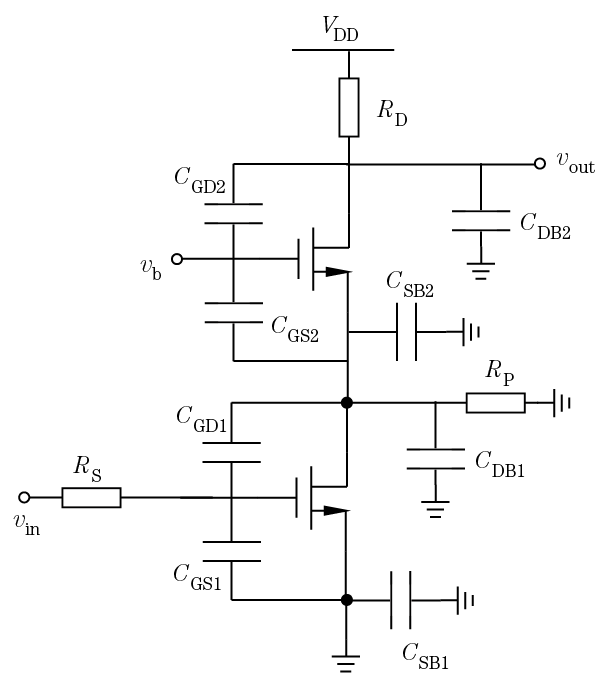
\includegraphics[width=1\textwidth]{p11-50-sol1.png}
        \caption*{(1) 标出电容}
        \end{minipage}
        \begin{minipage}[t]{0.433\textwidth}
        \centering
        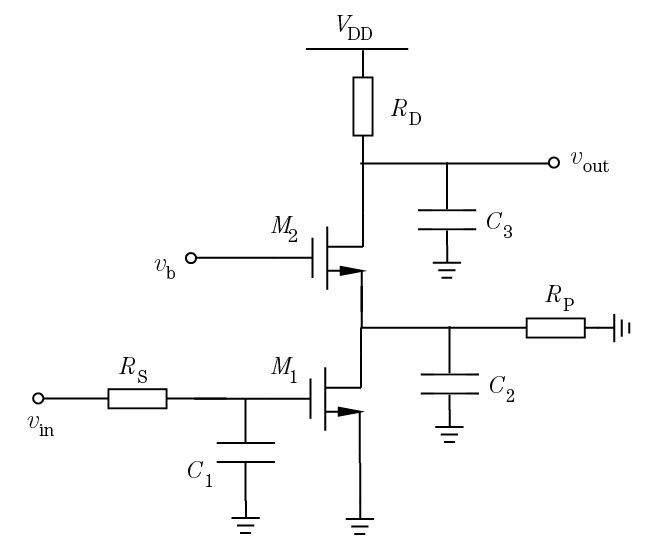
\includegraphics[width=1\textwidth]{p11-50-sol2.png}
        \caption*{(2) 简化电路}
        \end{minipage}
        \caption*{Figure 11-50}
    \end{figure}        
    \begin{align*}
        A_0 & = -g_{m1}g_{m2}R_D\left(\under{g_{m2} // R_P}\right) \\
        C_1 & = C_{GS1}+C_{GD1}\left(1+g_{m1}g_{m2}R_D\left(\under{g_{m2}} // R_P\right)\right) \\
        C_2 & = C_{SB2} + C_{DB1} + C_{GS2} + C_{GD1}\left(1+\under{g_{m1}g_{m2}R_D\left(\under{g_{m2} // R_P}\right)}\right) \\
        C_3 & = C_{DB2} + C_{GD2} 
    \end{align*}
    其中$A_0$为电路低频增益,从而
    \begin{align*}
        \omega_{p1} & = \left[ R_S 
            \left( C_{GS1}+C_{GD1}\left(1+g_{m1}g_{m2}R_D\left(\under{g_{m2}} // R_P\right)\right) \right)
            \right] ^ {-1} \\
        \omega_{p2} & = \left[ \left(\under{g_{m2}} // R_P\right)
            \left( C_{SB2} + C_{DB1} + C_{GS2} + C_{GD1}\left(1+\under{g_{m1}g_{m2}R_D\left(\under{g_{m2} // R_P}\right)}\right) \right)
            \right] ^ {-1}\\
        \omega_{p3} & = \left[ R_D
            (C_{DB2} + C_{GD2})
            \right] ^ {-1}\\
        A & = \frac{A_0}{
            \left( 1 + \frac{\J \omega}{\omega_{p1}}
            \right)
            \left( 1 + \frac{\J \omega}{\omega_{p2}} \right)
            \left( 1 + \frac{\J \omega}{\omega_{p3}} \right)
        }
    \end{align*}
\end{document} 